% ===========================================================================
% Master's thesis template
% Department of Engineering, University of Messina
% Supervisor: Prof. Francesco Longo
%
% HOW TO USE IT ON OVERLEAF
%   1. On overleaf.com: New Project > Upload Project > choose the .zip
%      downloaded from the website
%   2. Menu > Compiler: pdfLaTeX  (it is already the default)
%   3. Fill in the fields below and press Recompile
%
% References use BibTeX: entries go in bibliografia.bib and Overleaf runs
% bibtex by itself. Locally, several passes are needed:
%   pdflatex tesi && bibtex tesi && pdflatex tesi && pdflatex tesi
%
% The grey italic text inside the chapters is guidance: delete it as you write.
% ===========================================================================

\documentclass[12pt,a4paper,oneside]{report}

\usepackage[T1]{fontenc}
\usepackage{mathptmx}   % Times, as in the Word templates
\usepackage[utf8]{inputenc}
\usepackage[english]{babel}
\usepackage[a4paper,margin=3cm]{geometry}
\usepackage{graphicx}
\usepackage{float}   % [H]: figure e tabelle restano dove sono scritte
\usepackage{array}
\usepackage{setspace}
\usepackage{booktabs}
\usepackage{caption}
\usepackage{listings}
\usepackage{xcolor}
\usepackage[hidelinks]{hyperref}

\usepackage{remreset}
\makeatletter   % figure, tabelle e snippet numerati di seguito, non per capitolo
\@removefromreset{figure}{chapter}
\@removefromreset{table}{chapter}
\makeatother
\renewcommand{\thefigure}{\arabic{figure}}
\renewcommand{\thetable}{\arabic{table}}

\setlength{\parindent}{0pt}
\setlength{\parskip}{6pt}

\newcommand{\guidabib}{\guida{References are listed in the order in which they appear in the text and numbered: the number is the one you used to cite them in square brackets, and BibTeX takes care of that by itself. The style is IEEE, the one of the examples that follow — an article, a book and a web page — and it is applied by \texttt{ieeetr}, set in \texttt{tesi.tex}. The quickest way to collect the data is the «Cite» button on Google Scholar: ignore the styles it offers and take the BibTeX link at the bottom of the box, to paste into \texttt{bibliografia.bib}.}}
\makeatletter   % la bibliografia porta con se` titolo, voce d'indice e guida
\renewenvironment{thebibliography}[1]
  {\chapter*{\bibname}\addcontentsline{toc}{chapter}{\bibname}%
   \guidabib
   \list{\@biblabel{\@arabic\c@enumiv}}%
        {\settowidth\labelwidth{\@biblabel{#1}}%
         \leftmargin\labelwidth \advance\leftmargin\labelsep
         \@openbib@code \usecounter{enumiv}\let\p@enumiv\@empty
         \renewcommand\theenumiv{\@arabic\c@enumiv}}%
   \sloppy \clubpenalty4000 \@clubpenalty\clubpenalty
   \widowpenalty4000 \sfcode`\.\@m}
  {\def\@noitemerr{\@latex@warning{Bibliografia vuota}}\endlist}
\makeatother

\onehalfspacing
\newcolumntype{R}[1]{>{\raggedleft\arraybackslash}p{#1}}
\newcommand{\guida}[1]{{\itshape\color{gray}#1\par}}
\newcommand{\sugg}[1]{\nopagebreak\par\vspace{2pt}%
  {\normalfont\itshape\normalsize\color{gray}#1}}
\newcommand{\esempio}[1]{#1\par}
\setcounter{secnumdepth}{3}   % number subsubsections too
\setcounter{tocdepth}{3}      % and show them in the table of contents

\lstset{
  numberbychapter=false,
  numbers=left, numberstyle=\tiny\color{gray}, numbersep=8pt,
  basicstyle=\ttfamily\small, keywordstyle=\color{blue!60!black},
  commentstyle=\color{gray}, stringstyle=\color{green!40!black},
  frame=single, rulecolor=\color{gray!40},
  breaklines=true, showstringspaces=false, captionpos=b
}

% --- TO BE FILLED IN -----------------------------------------------------------
\newcommand{\corsodilaurea}{Master's Degree in \dotfill}
\newcommand{\titolotesi}{Title of the thesis}
\newcommand{\candidato}{Name Surname}
\newcommand{\relatore}{Prof. Francesco Longo}
\newcommand{\correlatore}{Prof. Name Surname}
\newcommand{\annoaccademico}{20\ldots/20\ldots}
% ---------------------------------------------------------------------------

\begin{document}

% ---------------------------------------------------------------------------
% Frontispiece. Compiling it on its own is useful per stamparlo e farlo firmare: il PDF
% firmato e` uno dei file da caricare su Esse3 con la domanda di laurea.
% Dentro la tesi non si compila da solo, viene incluso da tesi.tex.
% ---------------------------------------------------------------------------
\begin{titlepage}
  \centering

  
\includegraphics[width=3.2cm]{logo-unime.png}\\[0.7cm]
  {\Large\bfseries UNIVERSITY OF MESSINA}\\[0.25cm]
  {\large DEPARTMENT OF ENGINEERING}\\[0.35cm]
  {\large\bfseries \corsodilaurea}\\[0.12cm]
  \rule{\textwidth}{0.4pt}

  \vfill
  {\LARGE\bfseries \titolotesi}
  \vfill

  \begin{tabular}{@{}p{0.47\textwidth}@{\hfill}R{0.47\textwidth}@{}}
    Supervisor:              & Candidate:                \tabularnewline[0.15cm]
    \textbf{\relatore}       & \textbf{\candidato}       \tabularnewline[2cm]
    Co-supervisor:           &                           \tabularnewline[0.15cm]
    \textbf{\correlatore}    &                           \tabularnewline
  \end{tabular}

  \vspace{1.6cm}
  \rule{\textwidth}{0.4pt}\\[0.15cm]
  {\bfseries ACADEMIC YEAR \annoaccademico}

\end{titlepage}


\tableofcontents
\listoffigures
\listoftables

\chapter*{Abstract}
\addcontentsline{toc}{chapter}{Abstract}
\guida{Note for the whole thesis: you may use artificial intelligence tools to improve the form, the clarity and the correctness of the language, not to generate content, results or arguments that you would not be able to explain and defend.}
\guida{Note for the whole thesis: delete all the grey guidance from the final
version of your thesis.}
\guida{The abstract must be one page long and briefly describe the problem, what was done and the main result. Write it last, when you know what you obtained. It is also the summary to be deposited at the Segreteria didattica, which forwards it to the members of the examination board.}

\chapter{Introduction}
\guida{Every chapter opens with a paragraph announcing its content, outside
any section. A possible example is the following:}
\esempio{This chapter introduces the context in which the work is placed,
states the goal of the thesis and describes how the remaining chapters are
organised.}

\section{Context}
\guida{What this thesis is about and why the problem exists. Write it thinking of someone
who knows computer engineering but is not an expert in the subject of your
thesis.}

\section{Goal of the thesis}
\guida{What you set out to do. And above all what your contribution is, that
is what existed before and what exists now thanks to your work. It is the
first thing a committee looks for and the one students forget most often.}

\section{Structure of the thesis}
\guida{The map: one paragraph saying what each chapter contains, so that the
reader knows where to go.}

\chapter[Background]{Background \sugg{(change the title as you prefer)}}
\guida{One or more chapters. The criterion for deciding what belongs in these chapters is this: imagine a colleague has to continue your work and must read your thesis to do so. What do they need to know and study in order to understand what you did and how to carry it on? That is what goes in these chapters.}
\esempio{This chapter recalls the notions needed to follow the rest of the work: technology X, protocol Y and the techniques with which the literature addresses problem Z.}
\guida{Each chapter can be organised into several sections, each with several subsections and sub-subsections.}

\section{Title of the first section}
\guida{Sections, too, open by announcing their own content, in a single sentence. A possible example is the following:}
\esempio{This section describes technology X, from its execution model to the limitations that follow from it.}
\guida{This is also the chapter where almost all the sources appear. They are cited with a number in square brackets, at the end of the sentence before the full stop. A possible example is the following:}
\esempio{Container migration in fog computing has been studied by comparing the cold, pre-copy and post-copy techniques~\cite{esempio-articolo}. A systematic treatment of the algorithms involved can be found in~\cite{esempio-libro}, while the official runtime documentation describes the interface used here~\cite{esempio-web}.}
\subsection{Title of the subsection}
\guida{You go one level down when a section contains two or more topics that deserve a heading of their own. If there is only one, the subsection is not needed.}

\subsubsection{Title of the sub-subsection}
\guida{Third and last level. Any deeper and the numbering becomes unreadable: if you need it, it is better to rethink how the chapter is organised.}

\section{Title of the second section}

\subsection{Title of the subsection}

\subsubsection{Title of the sub-subsection}

\chapter[The work carried out]{The work carried out \sugg{(change the title to whatever best describes your own work)}}
\guida{One or more chapters, the core of the thesis. Explain your work in detail: the architecture of the system, software or algorithm you worked on, and the choices you made with their reasons.}
\esempio{This chapter presents the architecture of the system that was built, discusses its implementation choices and reports the experimental measurements that were collected.}
\guida{Each chapter can be organised into several sections, each with several subsections and sub-subsections.}

\section{System architecture}
\guida{Use many figures: think now about how you will give the presentation on the day of your graduation, and draw what you will explain out loud. For architecture and behaviour the most common UML diagrams are useful: activity, sequence and class diagrams.}

\guida{Every figure must be referred to in the text: a figure that is never cited is decoration. The caption goes below the figure. A possible example is the following:}
\esempio{The overall architecture of the system is shown in Figure~\ref{fig:esempio}.}

\begin{figure}[H]
  \centering
  
\includegraphics[width=4cm]{logo-unime.png}
  \caption{Caption of the figure.}
  \label{fig:esempio}
\end{figure}

\section{Software development}
\guida{Include only the listings that matter and explain the parts that count, the ones where an implementation choice is visible. Do not paste long portions of code: pick the ones that help the reader understand the work.}

\guida{Listings, too, must be referred to in the text: a listing that is never cited is decoration. The caption goes below the listing. A possible example is the following:}
\esempio{The function that computes the sum is shown in Listing~\ref{lst:esempio}.}

\begin{lstlisting}[language=C,caption={Caption of the listing.},label=lst:esempio]
int sum(int a, int b) {
    return a + b;
}
\end{lstlisting}

\section{Measurements and results}
\guida{Report every experimental measurement you managed to take and the observations that can be drawn from them about the efficiency and the performance.}
\guida{When the results come from repeatable measurements, run an adequate number of repetitions and report the variability as well, for instance the standard deviation or the confidence intervals. A mean with no indication of its variability says nothing about how far the comparison can be trusted.}

\guida{Tables, too, must be referred to in the text: a table that is never cited is decoration. The caption goes above the table. A possible example is the following:}
\esempio{The times measured in the two configurations are reported in Table~\ref{tab:esempio}.}

\begin{table}[H]
  \centering
  \caption{Caption of the table.}
  \label{tab:esempio}
  \begin{tabular}{lrr}
    \toprule
    Configuration & Average time (ms) & Standard deviation \\
    \midrule
    A & 12.4 & 0.8 \\
    B & 31.7 & 2.1 \\
    \bottomrule
  \end{tabular}
\end{table}

\guida{A chart is a figure to all intents and purposes, so it too must be referred to in the text and has its caption below. A possible example is the following:}
\esempio{The behaviour of the response time as the load grows is shown in Figure~\ref{fig:grafico}, where the vertical bars are the 95\% confidence intervals.}

\begin{figure}[H]
  \centering
  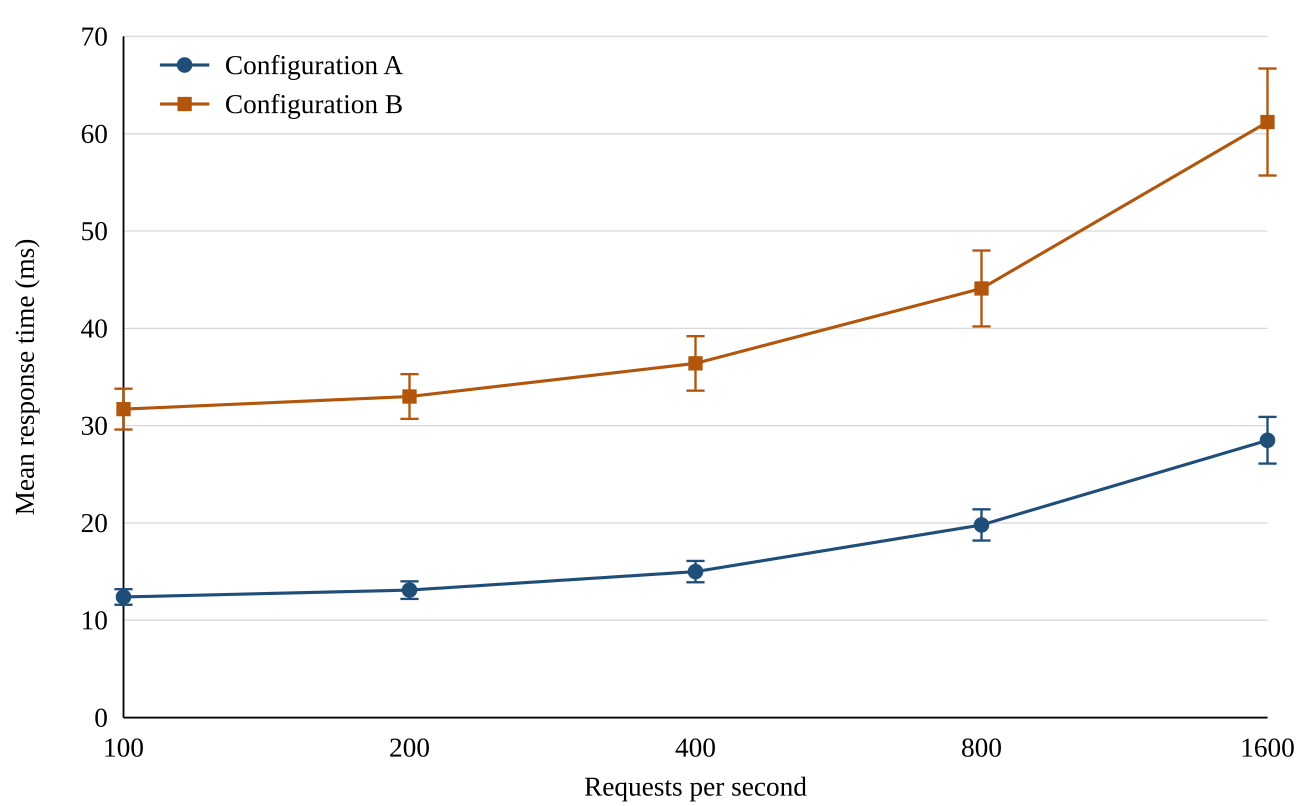
\includegraphics[width=11cm]{grafico.png}
  \caption{Mean response time as the load grows, with 95\% confidence intervals.}
  \label{fig:grafico}
\end{figure}

\chapter{Conclusions}
\guida{The last chapter, too, opens by announcing its own content.}
\esempio{This chapter summarises the results obtained, discusses their
limitations and indicates the directions in which the work can be continued.}
\guida{The conclusions introduce no new results and no new technical information: they interpret and summarise what the previous chapters have already presented. Summarise your results briefly. State the limits of the work as well: a thesis that acknowledges them is more credible, not less. Close with possible future developments, that is, where that colleague would start from.}

\bibliographystyle{ieeetr}
\bibliography{bibliografia}

\end{document}
